%
%  Template for writing APJ style papers
%
%  Created by Jordan Mirocha on 2009-09-17.
%  Copyright (c) 2009 . All rights reserved. (really? ha)
%

%%% Declarations
\documentclass[preprint2]{aastex}              % double-column, single-spaced document
%\documentclass[preprint2,longabstract]{aastex}% if abstract too long
%\documentclass[manuscript]{aastex}            % one-column, double-spaced document:

\usepackage{graphicx}
\usepackage{pslatex}
\usepackage{amsmath, amsthm, amssymb}
\usepackage{natbib}
\usepackage{epsfig}
\usepackage{appendix}

% Short names
\shorttitle{Optimized Multi-Frequency Spectra for Computational Radiative Transfer}
\shortauthors{Mirocha et al.}

%-------------------------------------- PAPER STARTS HERE --------------------------------------%

\begin{document}
    
%%% START custom commands
\newcommand{\HI}{\text{HI}}
\newcommand{\HII}{\text{HII}}
\newcommand{\HeI}{\text{HeI}}
\newcommand{\HeII}{\text{HeII}}
\newcommand{\HeIII}{\text{HeIII}}
\newcommand{\nHI}{n_{\text{HI}}} 
\newcommand{\nHII}{n_{\text{HII}}}  
\newcommand{\nHeI}{n_{\text{HeI}}}
\newcommand{\nHeII}{n_{\text{HeII}}}
\newcommand{\nHeIII}{n_{\text{HeIII}}}  
\newcommand{\dnHI}{dn_{\text{HI}}} 
\newcommand{\dnHII}{dn_{\text{HII}}}  
\newcommand{\dnHeI}{dn_{\text{HeI}}}
\newcommand{\dnHeII}{dn_{\text{HeII}}}
\newcommand{\dnHeIII}{dn_{\text{HeIII}}}  
\newcommand{\dt}{\text{dt}}
\newcommand{\nel}{n_{\text{e}}}  
\newcommand{\nb}{n_{\text{b}}}
\newcommand{\nnu}{$n_{\nu}$ }
\newcommand{\ncol}{n_i^{\text{col}}}
\newcommand{\gHI}{\Gamma_{\text{HI}}}  
\newcommand{\gHeI}{\Gamma_{\text{HeI}}}
\newcommand{\gHeII}{\Gamma_{\text{HeII}}}
\newcommand{\aHII}{\alpha_{\text{HII}}}  
\newcommand{\aHeII}{\alpha_{\text{HeII}}}  
\newcommand{\aHeIII}{\alpha_{\text{HeIII}}}
\newcommand{\bHI}{\beta_{\text{HI}}} 
\newcommand{\bHeI}{\beta_{\text{HeI}}}  
\newcommand{\bHeII}{\beta_{\text{HeII}}}  
\newcommand{\xHeII}{\xi_{\text{HeII}}}
\newcommand{\kB}{k_{\text{B}}}
\newcommand{\fheat}{f_{\text{heat}}}
\newcommand{\Lbol}{\mathcal{L}_{\text{bol}}}
\newcommand{\spec}{\mathcal{N}}
\newcommand{\Heat}{\mathcal{H}}
\newcommand{\trec}{$t_{\text{rec}}$}
%%% END custom commands

\title {Optimized Multi-Frequency Spectra for Numerical Radiative Transfer}
\author{Jordan Mirocha$^{\dagger}$, Stephen Skory, Jack Burns}
\affil{Center for Astrophysics and Space Astronomy, University of Colorado, Campus Box 389, Boulder, CO 80309}
\affil{NASA Lunar Science Institute, NASA Ames Research Center, Moffett Field, CA 94043, USA}
\email{$^{\dagger}$jordan.mirocha@colorado.edu}
\author{John Wise}
\affil{Georgia Institute of Technology}
\author{Steven Furlanetto}
\affil{University of California at Los Angeles}

%%%
%% Abstract
%%%
\begin{abstract}
The recent emergence and implementation of complex algorithms for radiative transfer in numerous cosmological hydrodynamics codes has led to a dramatic improvement in simulations of radiative feedback in various astrophysical environments.  However, due to computational expense, the spectra of radiation sources are often discretized into a small number of frequency bins.  Using simple 1D radiative transfer calculations around model stars and accreting black holes, we find that even in the idealized case of a static density field the reduction of continuous spectra to only a few discrete emission frequencies has significant consequences for the resulting temperature and ionization profiles.  We quantify the effects of different discretization schemes for objects of different luminosities and spectral models, and propose a new technique to reduce errors while minimizing computational expense.
\end{abstract} 
\subjectheadings {computational methods -- radiative transfer -- reionization -- radiative feedback}

%%%
%% Introduction
%%%
\section{INTRODUCTION}
The recent development of advanced numerical methods for radiative transfer has led to a substantial increase in the number of astrophysical problems that are computationally accessible.   Several fully 3D cosmological hydrodynamics codes have implemented adaptive ray-tracing methods (\cite{Abel2002}) for propagating radiation around point sources,  or flux-limited diffusion schemes (\cite{Reynolds2009}) for diffuse radiation fields.  More recently, hybrid-schemes have been implemented in smoothed-particle hydrodynamic codes (e.g. \cite{Petkova2011}).  For a review on the state of convergence among several widely used codes, see \cite{Iliev2006} and \cite{Iliev2009}.

Unfortunately, the vast majority of radiative transfer simulations run to date have only considered radiation at a single frequency.  While this monochromatic approach is the natural first step computationally-speaking, sampling radiation fields at multiple frequencies is essential for accurately calculating the properties of the medium through which photons propagate.  The mere presence of ionizing photons ensures that gas surrounding a radiation source will become ionized and heated, but the degree to which gas is ionized and heated depends on the total number of ionizing photons and their spectral energy distribution (SED).  As a result, we should expect the properties of gas surrounding a blackbody source of ultraviolet (UV) photons to be quite different from those of a power-law X-ray source such as an accreting black hole, for example.  Holding the bolometric luminosity of an object constant, even relatively small changes in SED can produce noticeable differences in surrounding gas properties, like changing the power-law index of a black-hole accretion spectrum (\cite{Kuhlen2005}; \cite{Thomas2008}).  But, these expectations are built on the assumption that each source is represented by a continuous SED, not one we have constructed with \nnu discrete frequency bins.  As we'll see in \S2, for a given source, the properties of the surrounding medium can be altered considerably solely due to the manner in which we discretize its spectrum.

The consequences of poor frequency resolution have been explored recently by \cite{Wise2011}, who find that for the expansion of an HII region around a $10^5$ K blackbody source in a hydrogen-only medium, the density, temperature, velocity, and ionization profiles are well converged for $n_{\nu} \ge 4$.  Use of a monochromatic spectrum for this problem introduces significant errors since all photons are absorbed at a characteristic column density, whereas multi-frequency treatments achieve some column density dependent behavior, and can thus mimic the behavior of a truly continuous spectrum.  The convergence for this test problem is reassuring, though the prospects for convergence are less clear if one were interested in the absorption processes of multiple chemical species, ionization and heating due to X-rays and their energetic secondary photo-electrons (\cite{Shull1985}; \cite{Furlanetto2010}), or inhomogeneous media.  Such effects are likely important in studies of radiative feedback from stars and active galactic nuclei (AGN), and most certainly in efforts to simulate cosmological reionization.  As a result, an effort must be made to ensure that the SEDs used to represent stars and black holes in numerical simulations actually reflect the behavior expected for those sources.  Additional motivation for this work comes from the fact that while spatial, temporal, and mass resolution for simulations are simple to calculate and straightforward to optimize, frequency resolution is not.  We aim to reduce the guesswork involved in discretizing SEDs, and provide a method for optimization on a problem-by-problem basis, just as one does for the other forms of resolution.

Though we will find that multi-frequency radiative transfer is necessary in most cases to accurately calculate the ionization and temperature state of the gas, it can also add significant computational expense.  Because the efficiency with which photons ionize and heat a gas depends on their energy, adding more energy groups will alter the amount of ionization and heating taking place in a given computational grid element.  But, these properties of the gas also dictate the computational time-step.  Generally, it is recommended that radiation time-steps are limited by a maximum fractional change in neutral species abundances so that ionization fronts are propagated at the correct speed (\cite{Shapiro2004}).  As a result, the addition of photons that ionize gas more efficiently will lead to a more expensive calculation since the time-step necessary to restrict changes in the neutral fraction will shrink.  Similarly, radiation-hydrodynamic simulations may be slowed by the inclusion of photons that heat gas efficiently, since higher temperature cells have greater sound speeds, and thus require a smaller time-step.  

Expense due to additional energy groups is certainly method-dependent, and may even be implementation-dependent.  For example, including high energy photons with long mean free paths will be very costly for a ray-tracing algorithm, but add no expense to a problem solved by flux-limited diffusion.  In addition, some adaptive ray-tracing implementations require each additional energy group in the source spectrum to be traced independently, in which case the time required by the radiative transfer solver scales roughly as \nnu.  Other implementations are now avoiding this problem by tracing all energy groups at once, though keeping them separate can be advantageous since energy groups with small mean free paths will be completely attenuated at small radii (\cite{Wise2011}).

With all of these factors in mind, we want to determine the following.  How many energy groups are required to adequately sample the true SED of a given radiation source?  Where should they be positioned in frequency?  What fraction of the bolometric luminosity should be allocated to each energy group?  What are the consequences of spectral discretization both physically and computationally?  

The contents of this paper fall into three general areas.  In \S2 we will quantitatively assess the accuracy with which multi-frequency calculations reproduce the ionization and heating profiles of continuous spectral energy distributions.  \S3 is devoted to introducing a technique for optimally selecting discrete SED templates so as to minimize the errors between discrete and continuous solutions, and \S4 will present the results obtained with this method.  In \S5, we conclude.  Verification of the code used for this work can be found in the Appendix.

%%% 
%% Multi-Frequency vs. Continuous
%%%
\section{ASSESSING THE CONSEQUENCES OF DISCRETE RADIATION FIELDS} \label{sec:Consequences}
Before computing the optimal multi-frequency spectra for SEDs most commonly used in numerical simulations (\S3), we will first demonstrate the difference in results brought about by varying degrees of frequency resolution.  To do this, we use \texttt{rt1d}, a 1D radiative transfer code developed for this work that is described and validated in the appendices.  

1D calculations were the natural choice for the problem at hand for a variety of reasons.  Since our sole focus is on the resolution dependence of radiative effects, it would be unnecessary to perform calculations in a more complex setting with additional unrelated physics.  In fact, doing so would likely make our results more opaque (ha).  Additionally, the algorithm of choice allows one to pre-tabulate the relevant ionization and heating quantities for a given radiation source, effectively allowing us to simulate sources with continuous SEDs.  Given our motives, this is clearly a necessary requirement.  Pre-tabulating key quantities also grants a significant speed-up for calculations that are already cheap, but most importantly, provides the basis for our optimization strategy that will be introduced in the next section.

In the remainder of this section, we will focus on two simple test problems.  First, the standard case of ionization and heating surrounding a $10^5$ K blackbody (problem \#2 in RT06), and second, the identical scenario for a power-law emitting X-ray source.  Initially, we will consider each case in a hydrogen-only medium, and later include the effects of helium.

\subsection{$10^5$ K Blackbody}



\subsection{Power-Law X-ray Source}

\begin{figure}[htbp]
\begin{center}
\includegraphics[scale=0.4]{figures/RT_Test1_RadialProfiles.ps}
\caption{this is a test.}
\label{fig:test}
\end{center}
\end{figure}








\section{METHODS} \label{sec:Methods}
Upon careful inspection of the coupled rate equations which govern the balance
of ionizations, recombinations, heating, and cooling, one realizes that the
integral values, i.e. equations \ref{eq:HIIRateEquation},
\ref{eq:HeIIRateEquation}, \ref{eq:HeIIIRateEquation}, and
\ref{eq:TemperatureEvolution} can be tabulated as a function of column density
(i.e. optical depth), allowing for a significant speed-up in run time. The key
to our subsequent analysis was inspired by this same convenient feature: if
$\Gamma_i$ and $\Heat_i$ can be tabulated for a given source
\textit{a-priori}, it means that \textit{precision determination of the
ionization state and temperature of the gas surrounding that source relies
solely on accurate numerical computation of the photoionization and heating
rate integrals in Equations \ref{eq:PhotoionizationRate} and
\ref{eq:HeatingRate}}. So, for a given source, we can compute the values of
these integrals numerically for the continuous spectrum, and then as discrete
sums given $n_{\nu}$ frequency bins with
\begin{equation}
    I(E) = \sum_{j=1}^{n_{\nu}} I(E_j) .
\end{equation}

% Optimization Strategy
\subsection{Optimization Strategy}
Our goal is to find the discrete spectrum, $I(E_j)$, that optimally reproduces the values of $\Gamma_i$ and $\Heat_i$ as a function of column density.  Denoting the photoionization and heating rates for a discrete spectrum as $\Gamma_i^d$ and $\Heat_i^d$, we want to minimize the difference between continuous and discrete solutions, i.e. $|\Gamma_i - \Gamma_i^d| = |\Heat_i - \Heat_i^d| = 0$.  As we will see in subsequent sections, these functions span several orders of magnitude in the ordinate over the column density regime of interest.  In order to place equal emphasis on the accuracy of solutions for high column densities (for which $\Gamma_i$ and $\Heat_i$ are small), it is more practical to seek solutions to
\begin{equation}
    \mathrm{log_{10}}\left | \frac{\Gamma_i}{\Gamma_i^d}\right | = \mathrm{log_{10}}\left | \frac{\Heat_i}{\Heat_i^d}\right | = 0 .
\end{equation}    
To do this, we employ a Monte-Carlo method called Simulated Annealing, in which we run $K$ Monte-Carlo trials, or random walks, each of which consists of $L$ steps.  In order to steer each random walk towards the global minimum, we will evaluate the quantity  
\begin{equation}
    P = \mathrm{exp}\left[-(f_{k,l} - f_{k,l-1}) / T \right]  \label{Probability}
\end{equation}
where $l=0,1,2,...L$ represents the current step in the current random walk, $k$, where $k = 0,1,2,...K$.  At each step in a given random walk, we generate a random number, $q$, that will determine whether we keep our current guess, $I(E_{k,l})$, or revert to our previous guess, $I(E_{k,l-1})$.  The condition for keeping our current guess is
\begin{equation}
    P \ge q .
\end{equation}
The key aspect of this analysis is how we vary the control parameter $T$, which is called the temperature in analogy with Boltzmann's equation.  Equation \ref{Probability} tells us that regardless of the value of $T$, if $f_l < f_{l-1}$ (i.e. our guess is better than the last), then
\begin{equation}
    P \ge 1
\end{equation}
and we have a 100\% chance of keeping our current guess.  It is clear now that how we control the temperature only effects how we deal with bad guesses (decreasing the temperature means we become less tolerant of bad guesses).  There are many ways of doing this, but for simplicity we adopt the following technique.  Every $m$ steps, we take
\begin{equation}
    T \rightarrow \gamma T ,
\end{equation}
where $\gamma$ is an experimentally determined quantity of order unity.


\section{RESULTS} \label{sec:Results}




\section{DISCUSSION}

% Could FLD methods tabulate? OTVET? RSPH?  MC?


\section{CONCLUSIONS}



\bibliography{references}
\bibliographystyle{apj}

%%% BEGIN APPENDIX
\appendix
\twocolumn
\appendixpage

%%% 
%% RT Framework
%%%
\section{RADIATIVE TRANSFER FRAMEWORK}
Our radiative transfer scheme is modeled closely after the work of \cite{Fukugita1994} and \cite{Thomas2008}, though for completeness we will reiterate here the aspects of these methods most pertinent to the problem at hand.  In general, propagating a radiation field relies on solving differential equations governing the rate of change in the number densities of all ions and the temperature of the gas.  Assuming a medium consisting of hydrogen and helium only, we first solve for the relative abundances of each ion via
\begin{align}
    \frac{d \nHII}{dt} & = \gHI \nHI + \bHI \nHI \nel - \aHII \nel \nHII   \label{eq:HIIRateEquation} \\ 
    \frac{d \nHeII}{dt} & = \gHeI \nHeI + \bHeI \nel \nHeI - \bHeII \nel \nHeII \nonumber \\ 
    & - \aHeII \nel \nHeII + \aHeIII \nel \nHeIII - \xHeII \nel \nHeIII  \label{eq:HeIIRateEquation} \\ 
    \frac{d \nHeIII}{dt} & = \gHeII \nHeII + \bHeII \nel \nHeII - \aHeIII \nel \nHeIII . \label{eq:HeIIIRateEquation}
\end{align}
Each of these equations represents the balance of ionizations and
recombinations for ions $\HII$, $\HeII$, $\HeIII$. We associate the index $i$
with neutral species, $i = \HI, \HeI, \HeII$, and define $\Gamma_i$ as the
photo-ionization rate coefficient, $\alpha_i$ ($\xi_i$) the case-A
(dielectric) recombination rate coefficients, $\beta_i$ the collisional
ionization rate coefficients, and $\nel$ the number density of electrons,
\begin{equation}
    \nel = \nHII + \nHeII + 2\nHeIII .
\end{equation}
In this work, we use the formulae in Appendix B of \citet{Fukugita1994} to compute the values of $\alpha$, $\beta$, and $\xi$.    We absorb ionizations due to to energetic photo-electrons into the  photoionization rate coefficients, $\Gamma_i$, which are given by
\begin{align}
    \Gamma_i = & \int_{E_i}^{\infty} \sigma_i(E) \spec(E) \frac{dE}{E} \nonumber \\  + & \sum_j f_i \left(\frac{n_j}{n_i}\right) \int_{E_i}^{\infty} \sigma_i(E)\left(\frac{E - E_j}{E_i}\right) \spec(E) \frac{dE}{E} \label{eq:PhotoionizationRate}
\end{align}
where $E_i$, $\sigma_i$, $n_i$, and $f_i$ are the ionization threshold energy, bound-free absorption cross section, number density, and fraction of photo-electron energy that goes into ionization of species $i$, respectively. The term summing over $j$, where $j = \HI, \HeI, \HeII$, represents ionizations of species $i$ due to fast secondary electrons from photoionizations of species $j$, which has number density $n_j$.  $\spec$ is the spectral intensity, which we write as
\begin{equation}
    \spec(E, r) = \frac{\Lbol}{4\pi r^2} I(E) e^{-\tau(E, r)} . \label{eq:Spectrum}
\end{equation}
Here, $r$ is the distance from the source, $I(E)$ is the normalized spectral energy distribution (SED), satisfying
\begin{equation}
    \int_E I(E) dE = 1 ,
\end{equation}
and the optical depth $\tau(E, r)$ is given as a sum over absorbing species,
\begin{align}
    \tau(E, r) & = \sum_i \int_r \sigma_i(E) n_i(r) dr \nonumber \\
               & = \sum_i \sigma_i(E) \ncol(r) \label{eq:OpticalDepth}
\end{align}
where $\ncol(r)$ is the column density of species $i$ at distance $r$ from the source.
We calculate the bound-free absorption cross-sections, $\sigma_i$, using the fits of \citet{Verner1996}.  At each time-step, we also solve for the temperature evolution, which is given by
\begin{align}
    \frac{3}{2}\frac{d}{dt}\left(\frac{\kB T \nb}{\mu}\right) & = \fheat \sum_i n_i \Heat_i \nonumber \\
    & - \sum_i \zeta_i n_e n_i - \sum_i \eta_i n_e n_i - \sum_i \psi_i n_e n_i \label{eq:TemperatureEvolution} 
\end{align}
where $\Heat_i$ is the photo-electric heating rate, given by
\begin{equation}
    \Heat_i = \int_{E_i}^{\infty} \sigma_i(E) \spec(E, r)(E - E_i) \frac{dE}{E} \label{eq:HeatingRate} ,
\end{equation}    
and $\zeta_i$, $\eta_i$, and $\psi_i$ are the collisional ionization, recombination, and collisional excitation cooling coefficients, respectively. The total number density of baryons is given by $\nb$, the mean molecular weight, $\mu$, Boltzmann's constant, $\kB$, the kinetic temperature of the gas, $T$, and the fraction of a photon's original energy deposited as heat, $\fheat$ (see \citet{Shull1985}, \citet{Furlanetto2010}).  For simplicity, our current treatment neglects cooling via free-free emission, as well as cosmological effects, including Hubble cooling due to cosmological expansion, Compton heating/cooling off cosmic microwave background (CMB) photons, and photo-ionization by Wien-tail CMB photons. 

It is important to note that we can pull radial and time dependencies outside of the integrals in Equations \ref{eq:PhotoionizationRate} and \ref{eq:HeatingRate}, leaving
\begin{equation}
    \Gamma_i(\ncol) = A \int_{E_i}^{\infty} \sigma_i(E) I(E) e^{-\tau(E, \ncol)} \frac{dE}{E} \
\end{equation}
and
\begin{equation}
    \Heat_i(\ncol) = A \int_{E_i}^{\infty} \sigma_i(E) I(E) (E - E_i) e^{-\tau(E, \ncol)} \frac{dE}{E}
\end{equation}
where $A \equiv \Lbol / 4 \pi r^2$.

It is now apparent that the values of $\Gamma_i$ and $\Heat_i$ can be tabulated as a function of column density for a given source.  This greatly improves the speed of 1D radiative transfer calculations, like those of \cite{Thomas2008}, since the integrals in these expressions (Equations \ref{eq:PhotoionizationRate} and \ref{eq:HeatingRate}) no longer need to be computed numerically on-the-fly.  It also provides the basis for our frequency resolution optimization strategy, as presented in \S\ref{sec:Methods}. Note, however, that the dimensionality of these lookup tables is equal to the number of absorbing species, so the tables for simulations including only hydrogen are 1D, and those including helium are 3D.

%%% 
%% Code Verification
%%%
\section{CODE VERIFICATION}
Our code, \texttt{rt1d}, solves Equations \ref{eq:HIIRateEquation}, \ref{eq:HeIIRateEquation}, \ref{eq:HeIIIRateEquation}, and \ref{eq:TemperatureEvolution} using the implicit Euler method for integration and the Newton-Raphson technique for root finding.  In order to track the propagation of ionization fronts accurately, we limit the time-step based on a maximum neutral fraction change as introduced in \citet{Shapiro2004},
\begin{equation}
    \Delta t = \epsilon_{\mathrm{ion}} \frac{\nHI}{|d\nHI/dt|} ,
\end{equation}
and additionally require that the time-step increase by a factor of two at most, as in \citet{Wise2011}.

%At this juncture it is worth mentioning the numerical artifacts that can result due to poor temporal or spatial resolution.  

% I-front evolution, RT06 #1
\begin{figure*}[htbp]
\centering
\includegraphics[scale=0.8]{figures/RT06_1_IfrontEvolution.eps}
\caption{\textit{Top:} Comparison of the numerical (dashed) and analytic (solid) solutions for the position of an expanding ionization front as a function of time in a hydrogen-only, isothermal medium (RT06 problem \#1).  The numerical solution displayed here is from the highest resolution simulation (6400 grid cells, i.e. $\Delta x = L_{\mathrm{box}}/6400$). \textit{Bottom:} Ratio of the calculated and analytic solutions as a function of time and grid resolution.  Simulations with $>$ 200 grid cells converge on the highest resolution solution to an accuracy of $\lesssim 5 \%$.}
\label{fig:RT_Test1_IfrontEvolution}
\end{figure*}

To demonstrate the functionality of the code, we repeat tests 1 and 2 from the Radiative Transfer Comparison Project (\cite{Iliev2006}; hereafter referred to as RT06).  Test 1 is the expansion of an HII region in a hydrogen-only, isothermal medium surrounding a monochromatic source of 13.6 eV photons. We adopt the parameters used in \citet{Wise2011}: constant temperature $T = 10^4 \ \mathrm{K}$, uniform hydrogen number density $n_H = 10^{-3} \ \mathrm{cm^{-3}}$, ionized fraction $x = 1.2 \times 10^-3$, in a box $L_{\mathrm{box}} = 6.6 \ \mathrm{kpc}$ in size, and with photon luminosity $\dot{Q} = 5\times10^{48} \ \mathrm{s^{-1}}$.  The classical analytic solution for the radius of an ionization front is 
\begin{equation}
    r_{\mathrm{IF}}(t) = r_s (1 - e^{-t/t_{\mathrm{rec}}})^{1/3}
\end{equation}    
where $r_s$ is the Str\"{o}mgren radius, 
\begin{equation}
    r_s = \left(\frac{3 \dot{Q}}{4\pi \alpha_{\mathrm{HII}}(T) n_{\mathrm{HI}}^2}\right)^{1/3} ,
\end{equation}
and the recombination time, \trec, is defined as
\begin{equation}
    t_{\mathrm{rec}} = \frac{1}{\alpha_{\mathrm{HII}}(T) n_{\mathrm{HI}}} .
\end{equation}
This solution is approximate even in isothermal media, given that it
assumes a constant neutral hydrogen density, $\nHI$. More accurate analytic
solutions exist (citations), and predict a departure from the classical
solution at $t/t_{\mathrm{rec}} \simeq 1$, which grows to a $\sim 5 \%$
difference by $t/t_{\mathrm{rec}} \simeq 4$. Our numerical solution (see
Figure \ref{fig:RT_Test1_IfrontEvolution}) captures this behavior very well.  In Figure \ref{fig:RT_Test1_RadialProfiles}, we show radial profiles of the ionized and neutral fractions at three stages of the I-front expansion, which are again in very good agreement with the calculations presented in \citet{Iliev2006}.

\begin{figure}[htbp]
\centering
\includegraphics[scale=0.4]{figures/RT_Test1_RadialProfiles.eps} 
\caption[]{Radial profiles of the neutral (solid) and ionized (dashed) fractions at $t = 10$, $30$, $100$, and $500$ Myr for Test 1.}
\label{fig:RT_Test1_RadialProfiles}
\end{figure}

Test 2 is the same as Test 1, except now the temperature is allowed to evolve according to Equation \ref{eq:TemperatureEvolution}, and the monochromatic radiation source is replaced by a $10^5$ K blackbody spectrum.  Radial profiles of the neutral and ionized fractions and temperature can be seen in the top and bottom panels of Figure \ref{fig:RT_Test2_RadialProfiles}, respectively.  Again, our numerical solutions are in very good agreement with previous work.

\begin{figure}[htbp]
\centering
\includegraphics[scale=0.4]{figures/RT_Test2_RadialProfiles.eps}
\caption{\textit{Top:} Radial profiles of the neutral (solid) and ionized (dashed) fractions at $t = 10$, $100$, and $500$ Myr. \textit{Bottom:} Radial profiles of the kinetic temperature at $t = 10$, $100$, and $500$ Myr (solid, dashed, and dotted lines, respectively).  Results in both panels from Test 2.}
\label{fig:RT_Test2_RadialProfiles}
\end{figure}

Still need to describe speed of light approximation, how the code is causal, etc.







\end{document}
